\documentclass[tikz,border=10pt]{standalone}
\usepackage{newtxtext,newtxmath} % 设置字体为 Times New Roman
\usetikzlibrary{shapes.geometric, arrows.meta, positioning, fit, calc}

\begin{document}
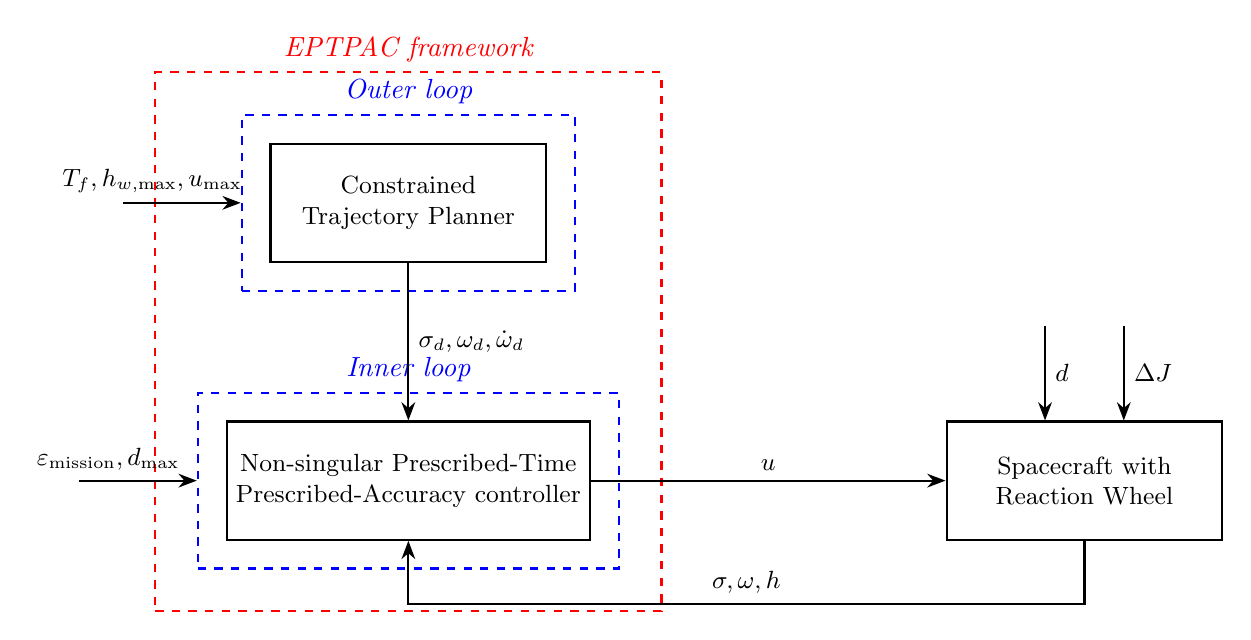
\begin{tikzpicture}[
    node distance=1.5cm and 2cm,
    every node/.style={font=\small},
    block/.style={rectangle, draw, thick, minimum width=3.5cm, minimum height=1.5cm, align=center},
    dashed_box/.style={rectangle, draw, dashed, thick, inner sep=10pt},
    red_dashed_box/.style={rectangle, draw=red, dashed, thick, inner sep=15pt},
    arrow/.style={-Stealth, thick}
]

% --- 主要模块节点 ---
\node (planner) [block] {Constrained \\ Trajectory Planner};
\node (controller) [block, below=of planner, yshift=-0.5cm] {Non-singular Prescribed-Time \\ Prescribed-Accuracy controller};
\node (spacecraft) [block, right=of controller, xshift=2.5cm] {Spacecraft with \\ Reaction Wheel};

% --- 内环与外环虚线框 ---
\node (outer_loop_box) [dashed_box, blue, fit=(planner)] {};
% 使用 \itshape 设置斜体
\node [blue, above, font=\itshape] at (outer_loop_box.north) {Outer loop};

\node (inner_loop_box) [dashed_box, blue, fit=(controller)] {};
\node [blue, above, font=\itshape] at (inner_loop_box.north) {Inner loop};

% --- 整体框架红框 ---
\node (framework_box) [red_dashed_box, fit=(outer_loop_box)(inner_loop_box)] {};
\node [red, above, font=\itshape] at (framework_box.north) {EPTPAC framework};

% --- 信号连接线 ---

% 外环输入
\draw [arrow] ($(outer_loop_box.west) - (1.5cm, 0)$) -- node[above, near start] {$T_f, \boldsymbol{h}_{w,\max}, \boldsymbol{u}_{\max}$} (outer_loop_box.west);

% 内环输入
\draw [arrow] ($(inner_loop_box.west) - (1.5cm, 0)$) -- node[above, near start] {$\varepsilon_{\mathrm{mission}}, \boldsymbol{d}_{\max}$} (inner_loop_box.west);

% 外环到内环
\draw [arrow] (planner.south) -- node[right] {$\boldsymbol{\sigma}_d, \boldsymbol{\omega}_d, \dot{\boldsymbol{\omega}}_d$} (controller.north);

% 控制器到航天器
\draw [arrow] (controller.east) -- node[above] {$\boldsymbol{u}$} (spacecraft.west);

% 反馈信号
\draw [arrow] (spacecraft.south) |- ++(0,-0.8cm) -| node[above, near start] {$\boldsymbol{\sigma}, \boldsymbol{\omega}, \boldsymbol{h}$} (controller.south);

% 外部扰动项 (包含 d 和 Delta J)
\draw [arrow] ($(spacecraft.north) + (-0.5cm, 1.2cm)$) -- node[right] {$\boldsymbol{d}$} ($(spacecraft.north) + (-0.5cm, 0)$);
\draw [arrow] ($(spacecraft.north) + (0.5cm, 1.2cm)$) -- node[right] {$\Delta\boldsymbol{J}$} ($(spacecraft.north) + (0.5cm, 0)$);

\end{tikzpicture}
\end{document}